\documentclass{standalone}

\usepackage{tikz}
\usetikzlibrary{positioning, calc, arrows.meta}
\usepackage{amsmath,amssymb}

\begin{document}
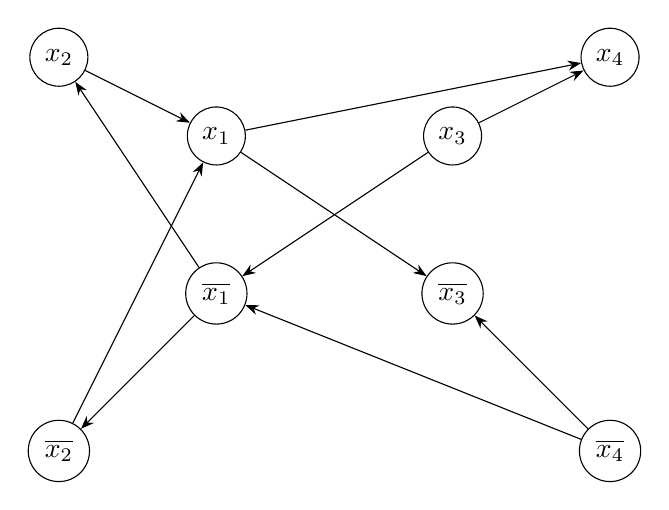
\begin{tikzpicture}[every node/.style = {draw, circle}, >=Stealth]
  \node[] (x2bar) {$\overline{x_2}$};
  \node[] (x2) at (0,5) {$x_2$};

  \node[] (x1bar) at (2,2) {$\overline{x_1}$};
  \node[] (x1) at (2,4) {$x_1$};

  \node[] (x3bar) at (5,2) {$\overline{x_3}$};
  \node[] (x3) at (5,4) {$x_3$};

  \node[] (x4bar) at (7,0) {$\overline{x_4}$};
  \node[] (x4) at (7,5) {$x_4$};

  \draw[->] (x2) -- (x1);
  \draw[->] (x1bar) -- (x2);
  \draw[->] (x2bar) -- (x1);
  \draw[->] (x1bar) -- (x2bar);
  \draw[->] (x1) -- (x3bar);
  \draw[->] (x3) -- (x1bar);
  \draw[->] (x3) -- (x4);
  \draw[->] (x4bar) -- (x3bar);
  \draw[->] (x1) -- (x4);
  \draw[->] (x4bar) -- (x1bar);
\end{tikzpicture}
\end{document}
